\documentclass[12pt]{article}
%\usepackage{fullpage}
\usepackage{epic}
\usepackage{eepic}
\usepackage{paralist}
\usepackage{graphicx}
\usepackage{algorithm,algorithmic}
\usepackage{tikz}
\usepackage{xcolor,colortbl}
\usepackage{wrapfig}


%%%%%%%%%%%%%%%%%%%%%%%%%%%%%%%%%%%%%%%%%%%%%%%%%%%%%%%%%%%%%%%%
% This is FULLPAGE.STY by H.Partl, Version 2 as of 15 Dec 1988.
% Document Style Option to fill the paper just like Plain TeX.

\typeout{Style Option FULLPAGE Version 2 as of 15 Dec 1988}

\topmargin 0pt
\advance \topmargin by -\headheight
\advance \topmargin by -\headsep

\textheight 8.9in

\oddsidemargin 0pt
\evensidemargin \oddsidemargin
\marginparwidth 0.5in

\textwidth 6.5in
%%%%%%%%%%%%%%%%%%%%%%%%%%%%%%%%%%%%%%%%%%%%%%%%%%%%%%%%%%%%%%%%

\pagestyle{empty}
\setlength{\oddsidemargin}{0in}
\setlength{\topmargin}{-0.8in}
\setlength{\textwidth}{6.8in}
\setlength{\textheight}{9.5in}


\def\ind{\hspace*{0.3in}}
\def\gap{0.1in}
\def\bigap{0.25in}
\newcommand{\Xomit}[1]{}


\begin{document}

\setlength{\parindent}{0in}
\addtolength{\parskip}{0.1cm}
\setlength{\fboxrule}{.5mm}\setlength{\fboxsep}{1.2mm}
\newlength{\boxlength}\setlength{\boxlength}{\textwidth}
\addtolength{\boxlength}{-4mm}
\begin{center}\framebox{\parbox{\boxlength}{{\bf
CS 4820, Spring 2018 \hfill Homework 1, Problem 1}\\
% TODO: fill in your own name, netID, and collaborators
Name: \\
NetID: \\
Collaborators:
}}
\end{center}
\vspace{5mm}

{\bf (1)} {\em (5 points)}\\
For any positive integer $n$, let $L_n$ denote
an L-shaped region in the plane obtained by starting
with a square of side length $2^n$ and deleting its 
upper right quadrant. For example, $L_1$ is the
``L-shaped tromino tile'' discussed in class on Wednesday.
See Figure~\ref{fig:L} for additional examples.
\begin{figure}[h]
  \centering
  \begin{minipage}{0.45\textwidth}
    \centering
    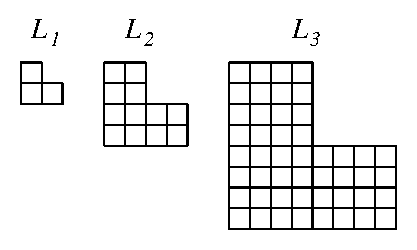
\includegraphics[width=\textwidth]{figl}
    \caption{The regions $L_1,L_2,L_3$}
    \label{fig:L}
  \end{minipage}
  \hfill
  \begin{minipage}{0.45\textwidth}
    \centering
    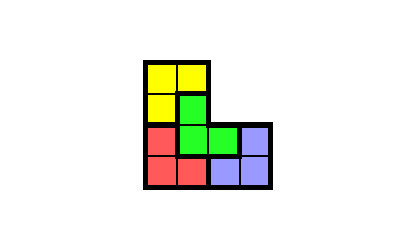
\includegraphics[width=\textwidth]{l2tile}
    \caption{Tiling $L_2$ with copies of $L_1$}
    \label{fig:l2tile}
  \end{minipage}
\end{figure}

\noindent
Prove, {\bf using mathematical induction,} that for every positive integer $n$ 
it is possible to tile $L_n$ using 
copies of $L_1$. In other words, you should
prove that $L_n$ can be partitioned into 
regions, each congruent to $L_1$.
See Figure~\ref{fig:l2tile} for an 
example when $n=2$.

Try to make your proof as clear and precise as 
possible. You do not need to 
describe an algorithm to compute the tiling, nor 
analyze its running time. You only must prove 
that such a tiling exists.

\vskip \bigap

%% Your solution goes here.

\end{document}
